% !TeX program = lualatex
\documentclass[]{article}

\usepackage{caption,subcaption,graphicx,float,url,amsmath,amssymb,amsthm,tocloft,cancel,thmtools,gensymb,braket,tikz-feynman,mathtools,color, colortbl}
\usepackage[toc,nonumberlist]{glossaries}
\usepackage{glossaries-extra}
\newcommand\numberthis{\addtocounter{equation}{1}\tag{\theequation}}

\newtheorem{thm}{Theorem}
\newtheorem{defn}[thm]{Definition}
\newtheorem{cor}[thm]{Corollary}
\newtheorem{lemma}[thm]{Lemma}
\graphicspath{{figs/}}
\widowpenalty10000
\clubpenalty10000
\setcounter{tocdepth}{2}
\tikzfeynmanset{compat=1.0.0}
\definecolor{Gray}{gray}{0.5}
%opening
\title{Theoretical Minimum\\Quantum Entanglement, Part 1}
\author{Simon Crase (compiler)\\simon@greenweaves.nz}

\begin{document}

\maketitle

\begin{abstract}
These are my notes from the Quantum Entanglement Part 1, lectures\cite{susskind2013entanglement}  from Leonard Susskind's Theoretical Minimum series\cite{susskind2007theoretical}. I have added headings based on the topics covered in each lecture, since each of the original lectures is has the same title, \emph{Quantum Entanglement}.

Disclaimer: I have created these notes as an aide-m\'emoire for my own use; if you find them useful, you are welcome, but I'd appreciate hearing from you. They are not intended 
as a substitute for listening to the lectures. The intellectual property for all material derived from the lectures belongs, of course, to Professor Susskind; any mistakes, however, are my own.

The notes were created using TexStudio\cite{TexStudio}, which I recommend for compiling them to a PDF; the bibliography was created using JabRef\cite{Jabref}.

\end{abstract}

\tableofcontents
\listoffigures
\listoftables
\listoftheorems


\section{Introduction}


We, as animals, have inherited, through the process of evolution, certain intuitive ways of thinking about the physical world:
\begin{enumerate}
	\item A lioness, pursuing an antelope, will stop as soon as relative velocity changes sign (physics calculation!);
	\item A Neanderthal pushing rock from door of cave aims body to maximize component of force in the right direction.
\end{enumerate}

Everything in modern physics has to do with those things that are beyond these intuitions:
speeds approaching speed of light; 4 D; the electron; the uncertainty principle. Why would natural selection have given us the intuition of the uncertainty principle? Intuitions for particles come from rocks.

This course will try to expose some of the weirdness of quantum mechanics, the weirdness of the logic of quantum mechanics, the weirdness of how quantum information works. 

This course will cover:
\begin{enumerate}
	\item the basic logic of quantum mechanics;
	\item the basic logic of quantum information theory
	\item physics as information.
\end{enumerate}

Classical mechanics represents values as real numbers; QM often uses discrete values. Before we cover quantum bits we will look at classical bits, using Dirac's notation $\ket{0}$ or $\ket{1}$--\cite{susskind2014quantum}. For an $n-bit$ \emph{classical} system, the number of configurations is $N_S=2^n$, so $n=\log_2(N_S)$.

We can generalize the definition of the number of bits of information: it doesn't have to be an integer. We can represent the state of a physical system, to a specified precision, by a string of bits (quantize space, etc). Figure \ref{fig:state_transition} shows how the laws of physics can be represented as a state transition diagram.

\begin{figure}[H]
	\caption[State transition diagram for laws of physics]{The laws of physics can be represented as a state transition diagram. In quantum mechanics there is no fundamental difference between forward in time and backward in time.}\label{fig:state_transition}
	\begin{subfigure}[t]{0.45\textwidth}
		\caption{Reversible Laws}\label{fig:state_transition_reversible}
		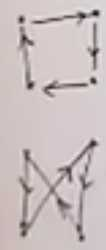
\includegraphics[width=0.8\textwidth]{et-1-1}
	\end{subfigure}
	\begin{subfigure}[t]{0.45\textwidth}
		\caption{An irreversible law}
		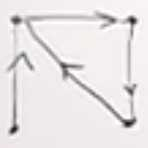
\includegraphics[width=0.8\textwidth]{et-1-2}
	\end{subfigure}
\end{figure}

All real systems are quantum mechanical. In this course we will try to answer the question why the quantum mechanics is suppressed in many systems we observe.

A Newtonian system is one that is in a definite state, and that evolves deterministically.

The Second Law of Thermodynamics arises because we lose the ability to follow the evolution of a system in precise detail.

LS reviews vectors and matrices:
\begin{itemize}
	\item Row and column vectors as sequences of number;
	\item Inner products;
	\item Matrices--linear transformation of vectors.
\end{itemize}

We can represent a state by a "one hot" vector, and then represent the transitions of, say, Figure \ref{fig:state_transition_reversible}, by a matrix of ones and zeros.

\section{Review of Quantum Mechanics}

This section reviews material from \cite{susskind2013quantum}.
\subsection{Spin of a single electron}

Classical mechanics is based on classical logic. Classical logic means that the states are Boolean: a set of points, each representing a state, and all the logic is classical. Quantum mechanics depends on a completely different logic.

We start with a quantum bit of Qbit, such as the spin of an electron.

We need the concepts of \emph{preparing} a state, and \emph{detecting} a state.

Classically we can \emph{prepare} an electron to point in a particular direction by placing it in a magnetic field. The electron will precess before aligning: the stronger the field the faster it emits electromagnetic radiation and aligns.

To \emph{detect} we apply magnetic field, and measure radiation to see how much realignmnet was needed.

This is \emph{not} the way a real electron works.

A real electron behaves like this. No matter how we prepare the electron, when we turn on the magnetic field, either:
\begin{itemize}
	\item nothing happens; or
	\item it emits a single photon corresponding to the flip from down to up.
\end{itemize}
It is almost as if the electron has only two possible configurations. But what if we prepare it at $45^\circ$ or $90^\circ$? Still we get up or down. What if we measure in some other direction?

What if we prepare up, turn off field, and later measure? Up.

What if we prepare at $45^\circ$, turn off field, then measure up/down? Then there is a probability of emitting photon. Probability has memory of previous state. Once you measure, state is fixed.

In physics we have learned not to ask questions unless we can devise a way to measure the answer.


\subsection{Spins of two Electrons}

\begin{itemize}
	\item The state space is an abstract vector space.

	\item LS reviews vector spaces, bras and kets, and represents the electron pointing up as $\ket{+}$. The general representation for an electron is $a_+\ket{+}+a_-\ket{-}$, where $a_+^*a_+$ is the probability that we will find the electron in the up state. Normalized vectors represent physical states.
	
	\item We have to rewire ourselves to understand QM.

	\item Linear combinations of states correspond to preparation in different directions.
	
	\item The two notions of vector (spatial and abstract) are related, but not simply.
	
	\item Anything that we can measure (with a number) is an observable.
	
	\item If we knew the rules for calculating averages for all possible observables, we would also know how to compute the probability distribution.
	
	\item Hermitian matrices are the quantum equivalent of observables.
	
\end{itemize}


\section{Postulates of Quantum mechanics}
\subsection{Review (continued)}
This section continues the review of material from \cite{susskind2013quantum}.

\begin{itemize}
	\item Complex numbers
	\item The equation $e^{i\theta} = \cos{\theta} + i \sin{\theta}$ contains all of trigonometry.
\end{itemize}

\subsection{Postulates of Quantum mechanics}

\begin{enumerate}
	\item States are represented by normalized vectors.
	\item Observables are represented by Hermitian matrices.
	\item $\braket{a|M|a}$ - expectation
	\item Eigenvalues and Eigenvectors
\end{enumerate}


We need complex numbers to handle evolution with time.

Define:
\begin{align*}
	\sigma_3 =& \begin{bmatrix} 1&0\\
	0&-1
                \end{bmatrix} \numberthis \label{eq:sigmas} \\
            \sigma_2 =& \begin{bmatrix}
            	0 & -i\\
            	i & 0
            \end{bmatrix}\\
     \sigma_1 =& \begin{bmatrix} 0&1\\
         	1&0
     \end{bmatrix} \text{, then}\\
	\sigma_3^2 =& 1 \numberthis \label{eq:sigma_sq}\\
	\sigma_3^2 =& 1\\
	\sigma_1^2 =& 1
\end{align*}
and the eigenvalues are $\pm1$.


\begin{thm}[If $M$ is Hermitian and it has two different eigenvalues, then the eigenvectors are orthogonal.]
	\begin{align*}
		M =& M^\dagger \text{ and} \numberthis \label{eq:hermitian}\\
		M \ket{a} =& \lambda_a \ket{a}\text{ and} \numberthis \label{eq:sigma_ev1}\\
		M \ket{b} =& \lambda_b \ket{b}\text{ and} \numberthis \label{eq:sigma_ev2}\\
		\lambda_a \ne& \lambda_b \numberthis \label{eq:ne} \\
		\implies&\\
		\braket{a \vert b} =& 0 \numberthis \label{eq:orthogonal}
	\end{align*}
\end{thm}

\begin{proof}
	From (\ref{eq:sigma_ev1})
	\begin{align*}
		\braket{b \vert M \vert a} =& \lambda_a \braket{b\vert a} \text{, similary from (\ref{eq:sigma_ev2})}\\
		\braket{a \vert M \vert b} =& \lambda_b \braket{a\vert b} \text{, or, using (\ref{eq:hermitian})}\\
		\braket{b \vert M \vert a} =& \lambda_b \braket{b\vert a} \text{, whence}\\
		(\lambda_1-\lambda_b)\braket{b\vert a} =& 0 \text{, so, using (\ref{eq:ne})}\\
		\braket{b\vert a} =& 0\text{, which is (\ref{eq:orthogonal})}
	\end{align*}
\end{proof}
\section{Spins \& Quantum Entanglement}

\subsection{Review of spins of single electrons (continued)}

Consider spin about an arbitrary "pointer" $(n_1,n_2,n_3)$

\begin{align*}
	\vec{\hat{n}}\cdot\vec{\sigma} =& n_1\sigma_1 + n_2\sigma_2 + n_3 \sigma_3\\
	=& \begin{bmatrix}
		n_3&n_1-i n_2\\
		n_1 + i n_2&-n_3
	\end{bmatrix}\\
\text{where }n_1^2 + n_2^2 +n_3^2 =& 1		
\end{align*}
We define:
\begin{align*}
	n_1-i n_2 =& n_-\\
	n_1+i n_2 =& n_+\text{ then}\\
	\vec{\hat{n}}\cdot\vec{\sigma} =&\begin{bmatrix}
		n_3&n_-\\
		n_+&-n_3 
	\end{bmatrix}\text{ an observable (turn on magnetic field along $\vec{n}$)}
\end{align*}
We can show that $(\vec{\hat{n}}\cdot\vec{\sigma})^2=I$, whence eigenvalues are $\pm 1$. Moreover
\begin{align*}
	n_+ n_- =& n_1^2 + n_2^2 + n_3^2 -n_3^2\\
	=& 1 - n_3^2
\end{align*}

Figure \ref{fig:et-4-1} depicts the only interesting question we can ask about a single spin: what if we prepare along one axis, measure along another, what is the probability of positive versus negative?

\begin{figure}[H]
	\caption{Prepare Spin along $\vec{\hat{n}}$, measure along $\vec{\hat{m}}$}\label{fig:et-4-1}
	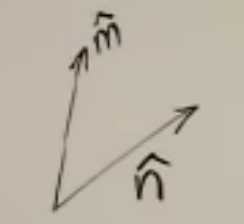
\includegraphics[width=0.8\textwidth]{et-4-1}
\end{figure}

We need the eigenvectors of $\vec{\sigma} \cdot \vec{\hat{n}}$ and   $\vec{\sigma} \cdot \vec{\hat{m}}$.
We have:
\begin{align*}
	(\vec{\sigma} \cdot \vec{\hat{n}}) \ket{\vec{\sigma} \cdot \vec{\hat{n}}=1} =& 1 \ket{\vec{\sigma} \cdot \vec{\hat{n}}=1} \text{ and}\\
	(\vec{\sigma} \cdot \vec{\hat{m}}) \ket{\vec{\sigma} \cdot \vec{\hat{m}}=1} =& 1 \ket{\vec{\sigma} \cdot \vec{\hat{m}}=1} \text{. We need the probability amplitude:}\\
	\vert \braket{\vec{\sigma} \cdot \vec{\hat{m}}=1\vert\vec{\sigma} \cdot \vec{\hat{n}}=1}\vert^2
\end{align*}

This is what quantum mechanics does: it answers the question, "What is the probability I'll get a measurement of this value, given that I prepared the experiment is such and such a manner?"

\begin{align*}
	\begin{bmatrix}
		n_3 &n_-\\
		n_+&-n_3
	\end{bmatrix}\begin{bmatrix}
		\alpha\\
		\beta
	\end{bmatrix}=&\begin{bmatrix}
		\alpha\\
		\beta
\end{bmatrix} \text{. WLOG}\\
	\begin{bmatrix}
	n_3 &n_-\\
	n_+&-n_3
\end{bmatrix}\begin{bmatrix}
	1\\
	z
\end{bmatrix}=&\begin{bmatrix}
	1\\
	z
\end{bmatrix} \text{, whence}\\
n_3 + n_- z =& 1\\
x =& \frac{1-n_3}{n-}
\end{align*}
 Normalizing:
 \begin{align*}
 	\ket{\vec{\sigma} \cdot \vec{\hat{n}}=1} =& \sqrt{\frac{1+n_3}{2}} \begin{bmatrix}
 		1\\\frac{1-n_3}{n_-}
 	\end{bmatrix}
 \end{align*}

Eventually we find:
\begin{align*}
	\vert \braket{\vec{\sigma} \cdot \vec{\hat{m}}=1\vert\vec{\sigma} \cdot \vec{\hat{n}}=1}\vert =& \frac{1 + \vec{\hat{n}} \cdot \vec{\hat{m}}}{2}\\
	=& \frac{1 + \cos{\theta_{mn}}}{2}
\end{align*}
We would get the same result if we rotated the experiment.

We can orient the system along any axis, and measure along any axis. We don't get fractional answers, we get fractional probabilities.

When you measure something, you go into system, interact with it, and \emph{change its state.} You leave the system in the eigenstate that corresponds to the measurement. Can we perform an experiment that measures spin along $\sigma_1$ and $\sigma_2$ simultaneously? No, because $\sigma_1$ and $\sigma_2$ don't share eigenvalues. For simultaneous measurement to be possible, need to share eigenvectors, i.e. if they \emph{commute}.

\begin{thm}[For simultaneous measurement to be possible, operators must commute.]
	\begin{align*}
			A\ket{\alpha_i} =& \lambda_i \ket{\alpha_i} \text{ and} \numberthis \label{eq:simultaneous1}\\
			B\ket{\alpha_i} =& \mu_i \ket{\alpha_i} \numberthis\label{eq:simultaneous2}\\
			\iff &\\
			AB - BA =& 0& \numberthis \label{eq:simultaneous3}\\
			[A,B] =& 0
	\end{align*}
\end{thm}

\begin{proof}
	From (\ref{eq:simultaneous1})
	\begin{align*}
		B A\ket{\alpha_i} =& \lambda_i B \ket{\alpha_i}\\
		=& \lambda_i \mu_i \ket{\alpha_i} \text{, from (\ref{eq:simultaneous2})} \text{. Similarly}\\
		A  B \ket{\alpha_i} =& \mu_i  lambda_i \ket{\alpha_i} \text{, whence}\\
		B A\ket{\alpha_i} =& A  B \ket{\alpha_i} \text{ for every eigenvector $\ket{\alpha_i}$}
	\end{align*}
\end{proof}
\begin{thm}[Any direction corresponds to an axis of spin.]
	For any $\alpha$ and $\beta$ such that $\alpha^2$ + $\beta^2=1$, there exista a direction of space such that $(\alpha, \beta)$ is an eigenvector of $\vec{\sigma} \cdot\vec{\hat{n}}$ with eigenvalue 1.
\end{thm}

\subsection{Pairs of electrons--Entanglement at last}
There are four states: $\ket{u\;u}, \,\ket{d\;u}, \,\ket{u\;d}, \,\ket{d\;d}$.  We will use $\sigma$ for the first electron, $\tau$ for the second:  $\sigma$ leaves the second spin unchanged, $\tau$ leaves the first unchanged.

How many ways to combine? 8-2 = 6, but this is more than we'd expect from $2\times2$! State space is richer than we'd expect. This is entanglement!

The following \emph{product state} corresponds to a situation where the first electron has been carefully placed in one state, and the second in another.
\begin{align*}
	\big[\alpha_1\ket{u} + \beta_1\ket{d}\big]\big[\alpha_2\ket{u} + \beta_2\ket{d}\big] =& \alpha_1 \alpha_2 \ket{uu} + \alpha_1 \beta_2 \ket{ud} + \beta_1 \alpha_2 \ket{du} + \beta_1 \beta_2 \ket{dd}
\end{align*}
In such a case, there is always one direction in which the spin of the first electron is up, and similarly for the second electron (generally a different direction). LS exhibited an example where this is not true.

\begin{align*}
	\frac{1}{\sqrt{2}}\big[\ket{ud}+\ket{du}\big] \numberthis \label{eq:T1}
\end{align*}

If one electron is up, the other is down, and vice versa. We can learn something about one electron by measuring the other!.

\begin{thm}[Any $\sigma_i$ or $\tau_i$ acts on the expression (\ref{eq:T1}) to give zero]
	\begin{align*}
		\big[\bra{ud}+\bra{du}\big]\sigma_i\big[\ket{ud}+\ket{du}\big]=&0 \text{ and}\\
		\big[\bra{ud}+\bra{du}\big]\tau_i\big[\ket{ud}+\ket{du}\big]=&0
	\end{align*}
\end{thm}

\begin{cor}
	$\vec{\sigma}\cdot\vec{\hat{n}}$ and $\vec{\tau}\cdot\vec{\hat{n}}$ both  act on the expression (\ref{eq:T1}) to give zero; hence the probability of a spin being $+1$ (or $-1$) along any axis is $\frac{1}{2}$.
\end{cor}

This is very different from two independent electrons.

\section{Bell's Theorem}

\subsection{Einstein-Podolsky-Rosen Correlation}

If we have two spins there are two interesting cases:
\begin{align*}
	\frac{1}{\sqrt{2}}\big[\ket{ud}\pm\ket{du}\big] \numberthis \label{eq:T1a}
\end{align*}
There is no way that either electron has a definite polarization. To see the difference between plus and minus in (\ref{eq:T1a}), consider the operator $\vec{\sigma} + \vec{\tau}$

\begin{align*}
\big(\vec{\sigma_z} + \vec{\tau_z}\big)\frac{1}{\sqrt{2}}\big[\ket{ud}\pm\ket{du}\big]=& 0\\
\big(\vec{\sigma_x} + \vec{\tau_x}\big)\frac{1}{\sqrt{2}}\big[\ket{ud}+\ket{du}\big]=& 2 \big[\ket{uu}+\ket{dd}\big]\\
\big(\vec{\sigma_x} + \vec{\tau_x}\big)\frac{1}{\sqrt{2}}\big[\ket{ud}-\ket{du}\big]=& 0\\
\big(\vec{\sigma_y} + \vec{\tau_y}\big)\frac{1}{\sqrt{2}}\big[\ket{ud}-\ket{du}\big]=& 0
\end{align*}
So, for the singlet state, $\frac{1}{\sqrt{2}}\big[\ket{ud}\pm\ket{du}\big]$, if we measure $\vec{\sigma}$ we know $\vec{\tau}$. (Einstein, Podolsky, Rosen)\cite{einstein1935can}

\subsection{Bell's Theorem and Bell's Inequality}\label{sec:bell}

We now come to Bell's famous theorem\cite{bell1964einstein}. Is it profound or trivial? Sometimes it seems profound, at other times it just seems to be a consequence of quantum mechanics. John Bell and Richard Feynman shared this ambivalence. The theorem is absolutely classical:  Bell's theorem excludes quantum mechanics; in quantum mechanics you can find violations of Bell's inequality.

NB: entanglement doesn't violate causality; we can't use it to send an instantaneous message from Alice to Bob. Bob has to receive a message from Alice in order to use his measurement.

\begin{thm}[Bell's Theorem]
We consider the class of objects that have certain properties $A$, $B$, and $C$.
	\begin{align*}
		N(A, \neg B) + N(B, \neg C) \ge N(A,\neg C)\text{,  Bell's inequality} \numberthis \label{eq:bell:inequality}
	\end{align*}
\end{thm}

Figure \ref{fig:bell} illustrates the theorem.
\begin{figure}[H]
	\caption{Venn Diagram for Bell's Inequality--\cite{wiki2020bell}}\label{fig:bell}
	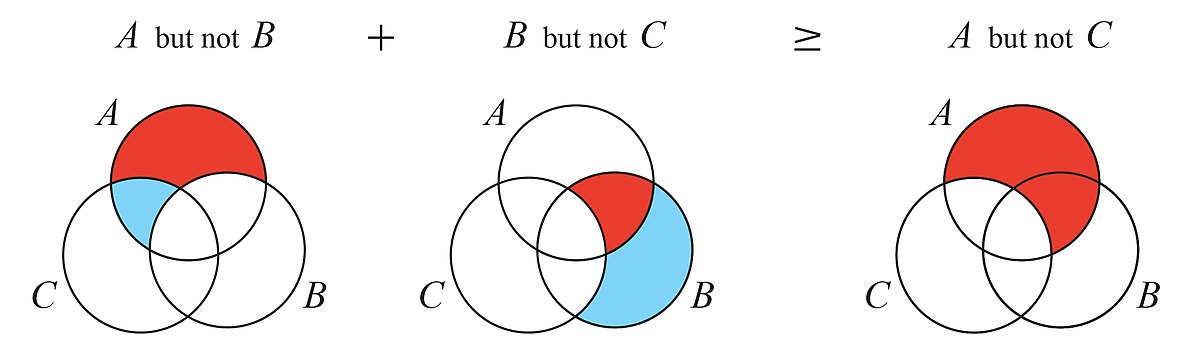
\includegraphics[width=0.8\textwidth]{1200px-Bell's_Theorem_JCB.jpg}
\end{figure}

\begin{proof}

    Table \ref{table:possibilities} depicts 8 possibilities for an object, which either has or does not have properties $A$, $B$, and $C$.
  
	\begin{table}[H]
		\caption[Bell's Theorem]{Bell's Theorem: each object either has or does not have properties $\{A, B,  C\}$. Each combination of properties is assigned a values chosen from the numbers 1 through 8. Finally, this table shows whether or not each combination contributes to the three sets $A \cap \neg B$, $B \cap \neg C$, and $A \cap \neg C $.}\label{table:possibilities}
		\begin{center}
			\begin{tabular}{|c|c|c|c|c|c|c|} \hline
				\#&$A$&$B$&$C$&$A \cap \neg B$&$B \cap \neg C$& $A \cap \neg C $\\ \hline
				\rowcolor{Gray}
				1&+&+&+&-&-&-  \\ \hline 
				2&+&+&-&-&+&+  \\ \hline
				3&+&-&+&+&-&-  \\ \hline 
				4&+&-&-&+&-&+  \\ \hline
				\rowcolor{Gray}
				5&-&+&+&-&-&-  \\ \hline 
				6&-&+&-&-&+&-  \\ \hline
				\rowcolor{Gray}
				7&-&-&+&-&-&-  \\ \hline
				\rowcolor{Gray} 
				8&-&-&-&-&-&- \\ \hline
			\end{tabular}
		\end{center}
	\end{table}

	From Table \ref{table:possibilities} we read off:
	\begin{align*}
		A \cap \neg B =& \{3, 4\} \\
		B \cap \neg C =& \{2, 6\} \text{, whence}\\
		(A \cap \neg B) \cup (B \cap \neg C) =&\{2,3,4, 6\}\\
		A \cap \neg C =& \{2,4\} \text{, from Table \ref{table:possibilities} }\\
		\subset& \{2,3,4, 6\} \text{, whence}\\
		A \cap \neg C \subset&(A \cap \neg B) \cup (B \cap \neg C)
	\end{align*}
Equation (\ref{eq:bell:inequality}) follows on taking the cardinalities of all three sets.
\end{proof}
What is amazing is that Bell's Inequality can be violated! One of the students said that the violation is profound. But all of QM violates classical mechanics. 

We now take our system to be two spins, and we will define $A$, $B$, and $C$. We will start by assuming classical spins, and that they can be measured as classical objects, and we will write down Bell's inequality. We will talk only about spin 1. A proposition might be: spin 1 is up along the z axis. The negative would be "spin 1 is not up along the z-axis, i.e. down", which is equivalent to "spin 2 is up" (in the Singlet state).

If classical logic made any sense we would measure (we have a beam of electron pairs. zillions of pairs, each of which are correlated) the first 100,000 in every possible manner, and we convince ourselves that the spins in each pair are opposite to each other. So the negative of "A is up" is "B is up."

\begin{table}[H]
	\caption{States for Classical Bell's inequality}\label{table:classical:bell}
	\begin{center}
		\begin{tabular}{|l|l|l|}\hline
			\#&Propositions& Negated\\ \hline 
			A&1 $\ket{u}$ along z axis&2 $\ket{u}$ along z axis\\ \hline
			B&1$ \ket{u}$ along $45^{\circ}$ angle in zx plane&2 $\ket{u}$ along $45^{\circ}$ angle in zx plane\\ \hline
			C&1 $\ket{u}$ along $90^{\circ}$ angle in zx plane&2  $\ket{u}$ along $90^{\circ}$ angle in zx plane\\ \hline
		\end{tabular}
	\end{center}
\end{table}

If the entities are pairs of electrons, the left hand side of (\ref{eq:bell:inequality}) becomes:
\begin{align*}
	\underbrace{N(A, \neg B)}_\text{1 up along z, 2 up along $45^\circ$} + \underbrace{N(B, \neg C)}_\text{N(A, \neg B) rotated $45^{\circ}$} =& 2N(A, \neg B)\text{ using rotational invariance of the Singlet.}
\end{align*}
The right hand side is 1 up along z, 2 up along $90^\circ$, so we have something we can test.
\begin{align*}
	2N(\text{1 up along z, 2 up along $45^\circ$}) \ge N(\text{1 up along z, 2 up along $90^\circ$}) \numberthis \label{eq:bell:ineq:classical}
\end{align*}
Note that we can replace numbers with probabilities, since we are working with zillions of electrons. When we calculate the probabilities for the singlet state, we find that the $\ge$ sign in (\ref{eq:bell:ineq:classical}) comes out <, violating Bell's inequality. To calculate efficiently, we require projection operators.

\begin{align*}
	\mathbb{P}_{\sigma_i} =& \frac{\sigma_i + I}{2} \text{, for $i \in \{1,2, 3\}$}
\end{align*}

\subsubsection{Alternative definition  for probability postulate of quantum mechanics}
If we have an arbitrary state $\psi$, and we want the probability that a certain thing is true, construct the projection operator for the eigenvector corresponding to that certain thing, $\mathbb{P}$; the probability is the expectation of $\mathbb{P}$, $\braket{\psi|\mathbb{P}|\psi}$.

\begin{enumerate}
	\item Projection operators correspond to statements.
	\item In classical physics, properties are subsets: the set of all things \emph{such that}...; we use classical logic.
	\item In quantum mechanics properties correspond to subspaces of a vector space; they are different from subsets of a set. 
\end{enumerate}

We'll recast Table \ref{table:classical:bell} in terms of projection operators.
\begin{table}[H]
	\caption{Projection operators for Bell's inequality}\label{table:projection:bell}
	\begin{center}
		\begin{tabular}{|l|l|l|l|}\hline
			\#&Proposition&Projection & Projection Negated\\ \hline 
			A& $\ket{u}$ along z axis&$\frac{1}{2}\big(\sigma_3 + I\big)$&\\ \hline
			B&$ \ket{u}$ along $45^{\circ}$ angle in zx plane&$\frac{1}{2}\big(\frac{\sigma_1+\sigma_3}{\sqrt{2}}+I\big)$&$\frac{1}{2}\big(\frac{\tau_1+\tau_3}{\sqrt{2}}+I\big)$\\ \hline
			C&$ \ket{u}$ along $90^{\circ}$ angle in zx plane&&$\frac{1}{2}\big(\tau_1+1\big)$\\ \hline
		\end{tabular}
	\end{center}
\end{table}

\subsubsection{Example calculation for violation of Bell's Inequality}

From Table \ref{table:projection:bell}, $P(A, \neg B) = \frac{1}{4}\big(\sigma_3 + I\big) \big(\frac{\tau_1+\tau_3}{\sqrt{2}}+I\big)$. Applying this to the Singlet, and using rotational invariance, the left side of (\ref{eq:bell:ineq:classical}) becomes:

\begin{align*}
	2& \frac{1}{\sqrt{2}}\big[\bra{ud}-\bra{du}\big]\frac{1}{4}\big(\sigma_3 + I\big) \big(\frac{\tau_1+\tau_3}{\sqrt{2}}+I\big)\frac{1}{\sqrt{2}}\big[\ket{ud}-\ket{du}\big]\\
	=& 2 \frac{1}{\sqrt{2}} \frac{1}{4} \frac{1}{\sqrt{2}} \big[\bra{ud}-\bra{du}\big]\big(\sigma_3 + I\big) \big(\frac{\tau_1+\tau_3}{\sqrt{2}}+I\big)\big[\ket{ud}-\ket{du}\big]\\
	=&\frac{1}{4} \big[\bra{ud}-\bra{du}\big]\big(\sigma_3 + I\big) \big(\frac{\tau_1+\tau_3}{\sqrt{2}}+I\big)\big[\ket{ud}-\ket{du}\big] \numberthis \label{eq:bell:lhs}
\end{align*}
We will build this expression up:
\begin{align*}
	\tau_3 \ket{ud} =& -\ket{ud}\\
	\tau_1 \ket{ud} =& \ket{uu}\\
	\tau_3 \ket{du} =& \ket{du}\\
	\tau_1 \ket{du} =& \ket{dd} \text{, whence}\\
	\big(\frac{\tau_1+\tau_3}{\sqrt{2}}+I\big)\ket{ud}=&\frac{\ket{uu}-\ket{ud}}{\sqrt{2}}+\ket{ud}\\
	=& \frac{\ket{uu}}{\sqrt{2}} + \big(1-\frac{1}{\sqrt{2}}\big)\ket{ud} \text{, and}\\
	\big(\frac{\tau_1+\tau_3}{\sqrt{2}}+I\big)\ket{du}=&\frac{\ket{dd}+\ket{du}}{\sqrt{2}}+\ket{du}\\
	=&\frac{\ket{dd}}{\sqrt{2}} + \big(1+\frac{1}{\sqrt{2}}\big)\ket{du}
\end{align*}
We now apply $\sigma_3 + I$:
\begin{align*}
	\big(\sigma_3 + I\big) \big(\frac{\tau_1+\tau_3}{\sqrt{2}}+I\big)\ket{ud}=&\big(\sigma_3 + I\big) \big[\frac{\ket{uu}}{\sqrt{2}} + \big(1-\frac{1}{\sqrt{2}}\big)\ket{ud}\big]\\
	=& 2 \big[\frac{\ket{uu}}{\sqrt{2}} + \big(1-\frac{1}{\sqrt{2}}\big)\ket{ud}\big] \text{, and}\\
	\big(\sigma_3 + I\big) \big(\frac{\tau_1+\tau_3}{\sqrt{2}}+I\big)\ket{du}=&\big(\sigma_3 + I\big) \big[\frac{\ket{dd}}{\sqrt{2}} + \big(1+\frac{1}{\sqrt{2}}\big)\ket{du}\big]\\
	=& 0
\end{align*}
So (\ref{eq:bell:lhs}) becomes:
\begin{align*}
	\frac{1}{4} \big[\bra{ud}-\bra{du}\big]  2 \big[\frac{\ket{uu}}{\sqrt{2}} + \big(1-\frac{1}{\sqrt{2}}\big)\ket{ud}\big] =& \frac{1}{2}\big(1-\frac{1}{\sqrt{2}}\big)\braket{ud|du}\\
	 =& \frac{1}{2}\big(1-\frac{1}{\sqrt{2}}\big) \numberthis \label{eq:bell:lhs:approx}
\end{align*}

Returning to Table \ref{table:projection:bell}, $P(A, \neg C) = \frac{1}{4}\big(\sigma_3 + I\big) \big(\tau_1+1\big)$. Applying this to the Singlet, and using rotational invariance, the right side of (\ref{eq:bell:ineq:classical}) becomes:
\begin{align*}
	\frac{1}{\sqrt{2}}&\big[\bra{ud}-\bra{du}\big]\frac{1}{4}\big(\sigma_3 + I\big) \big(\tau_1+I\big)\frac{1}{\sqrt{2}}\big[\ket{ud}-\ket{du}\big]\\
	=&\frac{1}{8}\big[\bra{ud}-\bra{du}\big]\big(\sigma_3 + I\big) \big(\tau_1+I\big)\big[\ket{ud}-\ket{du}\big] \numberthis \label{eq:bell:rhs}
\end{align*}

\begin{align*}
	\big(\tau_1+I\big) \ket{ud} =& \ket{uu} + \ket{ud}\\
	\big(\tau_1+I\big) \ket{du} =& \ket{dd} + \ket{du}\\
	\big(\sigma_3 + I\big) \big(\tau_3+I\big)\big[\ket{ud}-\ket{du}\big]=&
	\big(\sigma_3 + I\big) \big(\ket{uu} + \ket{ud}-\ket{dd} - \ket{du} \big)\\
	=& \ket{uu} + \ket{ud}+\ket{dd} + \ket{du} + \ket{uu} + \ket{ud}-\ket{dd} - \ket{du}\\
	=& 2 \big(\ket{uu} + \ket{ud}\big)
\end{align*}
So (\ref{eq:bell:rhs}) becomes:
\begin{align*}
	\frac{1}{8}\big[\bra{ud}-\bra{du}\big] 2 \big(\ket{uu} + \ket{ud}\big) =& \frac{1}{4}\braket{ud|ud}\\
	=&\frac{1}{4}
\end{align*}

Substituting this and (\ref{eq:bell:lhs:approx}) in (\ref{eq:bell:ineq:classical}), we get 
\begin{align*}
	\frac{1}{2}\big(1-\frac{1}{\sqrt{2}}\big) \ge &\frac{1}{4}\\
	2-\frac{2}{\sqrt{2}} \ge& 1\\
	1 \ge& \sqrt{2} \text{, a contradiction!}
\end{align*}

Thus the Singlet violates Bell's inequality: there is no possibility of an underlying classical way of thinking about QM where properties are based on set theory. It can not be the statistical theory of some underlying classical system, no matter how complicated, jumbled, or chaotic. 

\subsubsection{The Aspect Experiment\cite{aspect1982experimental}}
This is a beautiful experiment, which taught us a lot about measuring electrons, but the result was certain beforehand. Aspect asked whether there is an out, a way for classical mechanics to somehow simulate quantum mechanics: the answer is "yes", but only if the system under discussion has wires to connect the left electron to the right electron, so the electron on the left is not independent of the one on the right, and there is a processor in the centre. But the signals have to go faster than the speed of light! (Bob needs to tell Alice what is going on: what if the times are synchronized to the extent that the signals need to travel faster than light?) Aspect managed to check that the inequality was violated, and he did it in such a way that there was no way that light could have propagated between Alice and Bob to explain the results: that was the hard part of the experiment.

All attempts to simulate QM classically require signals to travel faster than the speed of light.

\subsection{The No-Cloning Theorem}

Evolution is linear. Imagine that a system moves from state $\ket{a}$ to $\ket{a^{\prime}}$ during time $t$, and from  $\ket{b}$ to $\ket{b^{\prime}}$. Then it moves from $\alpha \ket{a} + \beta \ket{b}$ to $\alpha \ket{a^{\prime}} + \beta \ket{b^{\prime}}$ during time $t$.

Let us suppose that we have a machine that will take a system in an arbitrary styate, and produce two systems that are in the exact same state--a cloning operation. A Xerox is a classical cloning machine.  Figure \ref{fig:quantum:cloning:machine} illustrates a quantum cloning machine.

\begin{figure}[H]
	\caption[Quantum Cloning machine: $\ket{u}\rightarrow \ket{u}\ket{u}$]{Quantum Cloning machine: $\ket{u}\rightarrow \ket{u} \ket{u}$. We'll use neutrons to avoid violating conservation of charge. (The machine supplies energy as needed.)}\label{fig:quantum:cloning:machine}
	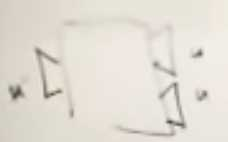
\includegraphics[width=0.8\textwidth]{quantum-cloning-machine}
\end{figure}

\begin{thm}[A quantum cloning machine is impossible]
\end{thm}

\begin{proof}
	 In order to prove that there a quantum cloning machine is impossible, we need merely exhibit one system that cannot be cloned.

	\begin{align*}
		\ket{u}\rightarrow& \ket{u}\ket{u}\\
		\ket{d}\rightarrow& \ket{d}\ket{d}\\
		\ket{r}\rightarrow& \ket{r}\ket{r} \text{, but } \numberthis \label{eq:no:clone:linear}\\
		\ket{r} =& \frac{\ket{u} + \ket{v}}{2} \text{, so linearity tell us}\\
		\frac{\ket{u} +\ket{v}}{2} \rightarrow&  \frac{\ket{u} \ket{u} + \ket{v} \ket{v}}{2} \text{. Does this agree with (\ref{eq:no:clone:linear})? (\ref{eq:no:clone:linear}) gives}\\
		\frac{\ket{u} +\ket{v}}{2}\rightarrow& \frac{\ket{u} +\ket{v}}{2} \frac{\ket{u} +\ket{v}}{2}\\
		\rightarrow& \frac{\ket{u}\ket{u} + \ket{u}\ket{d} + \ket{d}\ket{u}+\ket{d}\ket{d}}{4} 
	\end{align*}

\end{proof}

Our proof exploits the fact that cloning is quadratic, but time evolution is linear, to show that we can build a machine that clones $\ket{u}$ and $\ket{v}$, but not $\ket{r}$. There is some debate about building a machine to clone imperfectly: how good can it be?

\section{Bell's theorem and two-slit experiment}

\subsection{Questions about entanglement}

\begin{enumerate}
	\item What happens if one member of an entangled pair is caught by a black hole? The outside electron becomes entangled with the degrees of freedom of the black hole. When the black hole evaporates, the photons are entangled with the electron that was outside.
	\item What happens if two water molecules become entangled, and then one is placed in a bathtub full of water? The one outside becomes entangled with the state of the bathtub (the entangled molecule in the bathtub gets too mixed up with the others to have a clear identity). So what happens when the bathtub evaporates? The molecules remains entangled with the vapour, unless something comes over from the bathtub to interact with the molecules and break the entanglement. Disentanglement can take place, but only if the systems are close enough to interact.
	\item What happens when we measure two entangles particles? That takes them out. What if we measure only one? It can? These measurements are called "observations", and we'll talk about them during this lecture.
\end{enumerate}

\subsection{Subspaces and Projection Operator}

Review of several topics.
\begin{enumerate}
	\item Duality--bars and kets
	\item Orthogonality
	\item Linear Independence
	\item Dimension
\end{enumerate}

\begin{thm}[Basis vectors]
	In a $D$-dimensional space with orthogonality, we can always find $D$ mutually orthogonal, normalized basis vectors, $\ket{n} n=1,2,...D$.
\end{thm}

\begin{thm}[Expansion in basis vectors]
	Any state vector can be written:
	\begin{align*}
		\psi =& \sum_{n=1}^{D} a_n \ket{n} \text{, where}\\
		a_m =& \braket{m\vert\psi} \text{, and}\\
		\psi =& \sum_{n=1}^{D} \ket{n} \braket{n\vert\psi} \numberthis \label{eq:psi_expanded}
	\end{align*}
\end{thm}
Introducing the concept or a \emph{dyad}, $\ket{a}\bra{b}$:
\begin{align*}
	(\ket{a}\bra{b})\psi =& \ket{a}(\bra{b}\psi) \text{, we see from (\ref{eq:psi_expanded}):}\\
	\ket{n}\bra{n} =& I \text{, the "Resolution of the Identity"}
\end{align*}

We will derive some interesting subspaces: subspaces correspond to observable questions that we might ask. Imagine an observable $K$, and consider the eigenvalue/eigenvector:
\begin{align*}
	K \ket{a} =& \lambda \ket{a} \text{ Suppose there is a linearly independednt eigenvector with the same eigenvalue}\\
	K \ket{b} =& \lambda \ket{b} \text{, then any linearly independent combination is also an eigenvalue}\\
	K(\alpha \ket{a} + \beta \ket{b}) =& \lambda (\alpha \ket{a} + \beta \ket{b})
\end{align*}

There is a subspace corresponding to the eigenvalue. So the measurement $K=\lambda$ is not necessarily identified with a single vector, but with a subspace. Once you have identified a subspace, you can find a basis. Lets suppose we have found a basis, $\{\ket{a}, \ket{b}\},...$, with dimension $<D$ and construct $\sum_a \ket{a} \bra{a}$

\begin{align*}
	(\sum_a \ket{a} \bra{a}) \psi =& \psi \text{, if $\psi$ in subspace}\\
	=& \text{ projection onto subspace otherwise}\\
	\sum_a \ket{a} \bra{a} =& \mathbb{P}_{K=\lambda} \numberthis \label{eq:projection}
\end{align*}

To construct a projection operator for a values of a property:
\begin{enumerate}
	\item find subspace;
	\item find basis in that subspace;
	\item construct what would have been the identity--(\ref{eq:projection}).
\end{enumerate}
Any projection operator characterizes a property--the property that is true in that subspace.

The probability postulate for quantum mechanics is most nicely expressed in terms of projection operators. Given an arbitrary, normalized, state $\psi$, which may or may not be in the subspace, the probability that $K$ has value $\lambda$ is the expectation $\braket{\psi\vert\mathbb{P}_{K=\lambda}\vert\psi}$

\begin{align*}
	\braket{\psi\vert\mathbb{P}_{K=\lambda}\vert\psi}=&\sum_a \braket{\psi\vert a}\braket{a \vert \psi} \text{, e.g.}\\
	\mathbb{P}_\text{first spin up}=&\ket{uu}\bra{uu} + \ket{ud}\bra{ud}
\end{align*}

Two \emph{commuting} projection operators, $\mathbb{P}_{K=\lambda}$ and $\mathbb{P}_{L=\mu}$ enable simple definitions or "and" and "or" (we assume that the subspaces have non-zero vectors in common).

\begin{thm}[Commuting projection operators]\label{thm:commuting}
	If $\mathbb{P}_{K=\lambda}$ and $\mathbb{P}_{L=\mu}$ commute:
	\begin{align*}
		\mathbb{P}_{K=\lambda \land L=\mu} =& \mathbb{P}_{K=\lambda}\mathbb{P}_{L=\mu}\\
		\mathbb{P}_{K=\lambda \lor L=\mu} =& \mathbb{P}_{K=\lambda} + \mathbb{P}_{L=\mu}
	\end{align*}
\end{thm}

\begin{proof}
	\begin{align*}
		K (\mathbb{P}_K\ket{\psi}) =& \lambda (\mathbb{P}_K\ket{\psi}) \text{\because $\mathbb{P}_K\ket{\psi}$ subspace of things with property K}\\
		\mathbb{P}_K\mathbb{P}_L \ket{\psi} =& \mathbb{P}_L\mathbb{P}_K \ket{\psi} \text{, has properties K \& L}
	\end{align*}
	So $\mathbb{P}_K\mathbb{P}_L$ corresponds to K \& L.
\end{proof}

Spins operators for two particles, $\sigma_i$ and $\tau_j$, are compatible.

\subsection{Bell's theorem review}\label{sec:bell:review}

NB: Bell not always violated. It is often true for some properties, not others. 

In Section \ref{sec:bell}, we saw from (\ref{eq:bell:inequality}), that, for a classical system $$N(A, \neg B) + N(B, \neg C) \ge N(A,\neg C)$$
We consider a two electron system with spins:
\begin{itemize}
	\item A $\uparrow$;
	\item B $\nearrow$;
	\item C $\rightarrow$.
\end{itemize}
Negating a property for one electron is the same as asserting it for the other electron if system is a Singlet. We can recast (\ref{eq:bell:inequality}):
$$N(\uparrow \nearrow) + N(\nearrow \rightarrow) \ge N(\uparrow\rightarrow)$$
Or, in terms of projection operators.
\begin{table}[H]
	\begin{center}
		\caption{Recast (\ref{eq:bell:inequality}) in terms of projection operators, using Theorem \ref{thm:commuting}}
		\begin{tabular}{|c|c|c|} \hline
			$\uparrow\nearrow$&$\nearrow\rightarrow$&$\uparrow\rightarrow$ \\ \hline
			$\frac{1+\sigma_3}{2} \Big(\frac{1+\frac{\tau_1+\tau_3}{\sqrt{2}}}{2}\Big)$&$\Big(\frac{1+\frac{\sigma_1+\sigma_3}{\sqrt{2}}}{2}\Big)\frac{\tau_1+1}{2}$&$\frac{1+\sigma_3}{2} \frac{1+\tau_1}{2}$ \\ \hline
		\end{tabular}
	\end{center}
\end{table}


\url{https://youtu.be/xXBx8_19nyw?t=3836}

\subsection{Two slit and interference} 

\subsection{Measurement and entanglement in the two-slit experiment}

\section{Quantum Entanglement}

\subsection{Two slit interference and measurement} 

\subsection{High energy electrons emitting photons and destroying interference without explicit measurement} 

\subsection{Schr\"odinger cat and Wigner's friend} 

 \subsection{Entropy, level of entanglement}  
 
 \subsection{Trace and Density matrix }
 
\section{Entropy \& Dynamics}

\subsection{Entropy and Density matrix; Measuring Entanglement Entropy} 

\subsection{Subsystems in pure states}

\subsection{Entropy is not additive}

\subsection{Dynamics in time - Schr\"odinger equation}

\subsection{Unitary operators}

\subsection{Hamiltonian}

\section{Quantum Entanglement}

\subsection{Dynamics of states in time; Hamiltonian is Energy}

\subsection{Commutators, conservation}

\subsection{Mixed state of energy}

\subsection{Spin in a magnetic field}

\subsection{Singlet vs Triplet states}

\bibliographystyle{unsrt}
\addcontentsline{toc}{section}{Bibliography}
\raggedright
\bibliography{tm}

\end{document}
